\documentclass{article}

\usepackage{amssymb,amsmath,amsfonts,amstext}
\usepackage{graphicx}
%\usepackage{subfigure}
\usepackage{mathtools}
\usepackage{stmaryrd}
\usepackage{color}
\usepackage{verbatim}
\usepackage{amsthm}
\usepackage{esint}
\usepackage{caption,subcaption}
\usepackage{titlesec}
\setcounter{secnumdepth}{4}
\usepackage{geometry}
\geometry{left=3.18cm,right=3.18cm,top=2.54cm,bottom=2.54cm}


\title{Convolutional neural networks}
\author{Xiaoguai Li}
\date{}

\begin{document}


\maketitle


Train convolutional neural networks by Pytorch to do image recognition. Figure.1 shows the relation between number of epochs and loss. According to this plot, loss converges to a small value when number of epochs is large enough. All parameters and settings are consistent with what are mentioned in the problem description.  After 20 epochs, confusion matrix is obtained as 
\[
\begin{bmatrix}
1001  &  0 &   2   & 0   & 2    &0    &0   & 0   & 0 &   0\\
    1 & 972  &  0&    0&    0  &  0  &  0 &   0 &   1 &   0\\
   0  &  0& 1030   & 1   & 0   & 1  &  0  &  0   & 0  &  0\\
    0   & 0  &  0 &1014  &  0   & 2   & 0 &   0  &  0&    0\\
    0  &  0 &   0  &  3  &996 &   0  &  0   & 0 &   0 &   0\\
    0  &  0    &1  &  4    &2 & 929   & 0  &  1  &  0 &   0\\
    0    &0    &1  &  5    &2   & 0 &1021 &   1&    0 &   0\\
    0   & 0&    2&4    1 &   1  &  0  &993 &   0  &  0\\
    0    &1  &  0   & 1 &   1  &  0 &   0 &   0& 1022  &  0\\
    2    &1&    0  &  2 &   1 &   1  &  0 &   0  &  3  &971
\end{bmatrix}. 
\]
Test Accuracy of the model on the 10000 test images: 99 \%.
The main script is 'imageRecognition.py'. CNN model is realized in 'models\_pytorch\_CNN.py'.

\begin{figure}[h]
    \center
    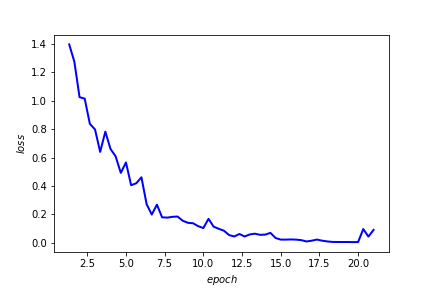
\includegraphics[width=0.5\textwidth]{loss2}
    \caption{Loss decreases with increasing number of epochs}
\end{figure}



\end{document}



